\section{システム使用例}\label{sec:4}%%%システム使用例じゃなくてテストという単語を入れてもいいかも
%\ref{sec:4}では実際にシステムを動かした際の詳細を書く\par
本章では、Desharnaisデータセット\cite{Desharnais89}(表\ref{table:DesharnaisDataset})を用いたSDepT v2.0.0のシステム使用例を示す.
Desharnaisデータセットは1980年代のカナダのソフトウェア開発会社のプロジェクトデータが記録されており,81件の過去のプロジェクトデータと11のプロジェクト特性(チームの経験年数(TeamExp in years),開発年度(YearEnd),マネージャーの経験年数(ManageExp in years),開発年数(Length),トランザクション数(Transactions),エンティティ数(Entities),調整済みファンクションポイント(PointsAdjust),調整係数(Envergure),未調整ファンクションポイント(PointsNonAdjust),開発言語(Language),開発工数(Effort))が含まれている.
\begin{table*}[ht]
  \centering
  \captionsetup{labelformat=empty} % 図番号を非表示に設定
  \caption{\Tdualcaption{A Sample Dataset of Software Development.}{Desharnaisデータセット.}}
  \label{table:DesharnaisDataset}
  \begin{center}
    \resizebox{\textwidth}{!}{
      \begin{tabular}{|c|c|c|c|c|c|c|c|c|c|c|c|}
        \hline
        Project & TeamExp & ManagerExp & YearEnd & Length & Transactions & Entities & PointsAdjust & Envergure & PointsNonAjust & Language & Effort \\ \hline \hline
        1 & 1 & 4 & 85 & 12 & 253 & 52 & 305 & 34 & 302 & 1 & 5152 \\ \hline
        2 & 0 & 0 & 86 & 4 & 197 & 124 & 321 & 33 & 315 & 1 & 5635 \\ \hline
        3 & 4 & 4 & 85 & 1 & 40 & 60 & 100 & 18 & 83 & 1 & 805 \\ \hline
        \vdots & \vdots & \vdots & \vdots & \vdots & \vdots & \vdots & \vdots & \vdots & \vdots & \vdots & \vdots \\ \hline
        80 & 4 & 3 & 86 & 12 & 469 & 176 & 645 & 43 & 697 & 3 & 5880 \\ \hline
        81 & 4 & 4 & 85 & 36 & 886 & 241 & 1127 & 34 & 1116 & 1 & 23940 \\ \hline
      \end{tabular}
    }
  \end{center}
\end{table*}


% \begin{table}[h]
%   \centering
%   \caption{Desharnaisデータの特性一覧}
%   \label{table:Desh}
%   \begin{tabular}{|c|c|} \hline
%     チームの経験年数(TeamExp in years) & 開発年度(YearEnd) \\ \hline
%     マネージャーの経験年数(ManageExp in years) & 開発年数(Length) \\ \hline
%     トランザクション数(Transactions) & エンティティ数(Entities) \\ \hline
%     調整済みファンクションポイント(PointsAdjust) & 調整係数(Envergure) \\ \hline
%     未調整ファンクションポイント(PointsNonAdjust) & 開発言語(Language) \\ \hline
%     開発工数(Effort) & ~ \\ \hline
%   \end{tabular}
% \end{table}

\subsection{ユーザーインターフェース}
ユーザーは以下の手順で操作を行う.
\begin{enumerate}
  \item 「Upload」ボタンを押し,ユーザーデータセットをアップロードする.
  このとき,アップロードしたデータセットのファイル名が「Upload」ボタンの横に表示されていれば,正常にアップロードされている.
  また,データセットがアップロードされていない場合はサンプルデータセットとして「sampleData.csv」が使用される.
  \item \begin{itemize}
    \item Basic画面では,予測精度を優先するか,計算速度を優先するかを選択できる.
    \item Advance画面では,各工程における採用手法を選択することができる.類似プロジェクト選定手法については,クラスタリングにおけるクラスタ数$k$,Fixed-kにおける選択プロジェクト数$k$,四分位数法における選択集合数$k$をそれぞれ任意に設定することができ,設定しなかった場合はデフォルトの数値で予測が行われる.
    \end{itemize}
  \item 「Predict」ボタンを押すことで予測が始まる.
  \item 計算が終了し画面が切り替わると,「Download」ボタンを押して予測結果をcsv形式でダウンロードすることができる.

\end{enumerate}

\subsection{予測結果レポート}
開発工数の予測が完了すると,予測結果として新規プロジェクトの工数予測値,各手法の予測精度,新規プロジェクトに対する類似プロジェクト,VIF値がそれぞれcsvファイルとして返される.
実際には,前処理の組み合わせごとに最大16組(欠損値補完4手法$\times$正規化4手法)のレポートが返されるが,ここでは例として,中央値による欠損値補完及びZ-score正規化を施したデータの出力レポートを表\ref{table:est}~表\ref{table:vif}に示す.

\begin{table*}[ht]
  \centering
  \captionsetup{labelformat=empty} % 図番号を非表示に設定
  \caption{\Tdualcaption{``Predicted Effort for New Project" Report.}{新規プロジェクトの工数予測値.}}
  \label{table:est}
  \resizebox{\textwidth}{!}{
    \begin{tabular}{|l|r|r|r|r|r|r|r|r|}
      \hline
        ~ & OLS & Ridge & Lasso & ElasticNet & SCAD & MCP & AdaptiveLasso & NonNegativeGarrote \\ \hline
        ED-Clustering($k$=2) & 32084  & 14345  & 11868  & 12046  & 13481  & 13610  & 10924  & 19878  \\ \hline
        ED-Clustering($k$=3) & 10710  & 7149  & 28993  & 27931  & 3859  & 30606  & 19180  & 20900  \\ \hline
        ED-Clustering($k$=4) & -12352  & 5199  & 17626  & 15766  & 3399  & 3399  & 14332  & 17095  \\ \hline
        ED-Clustering($k$=5) & -12352  & 5199  & 17626  & 15766  & 3399  & 3399  & 14332  & 17095  \\ \hline
        ED-Fixed\_$k$($k$=3) & -6511  & 7132  & 4335  & 11471  & 4736  & 4717  & 6271  & 6513  \\ \hline
        ED-Fixed\_$k$($k$=4) & -23068  & 6749  & 7903  & 11635  & 4253  & 4253  & 7388  & -36596  \\ \hline
        ED-Fixed\_$k$($k$=5) & -19520  & 4536  & 9791  & 9921  & -33173  & -24506  & 4618  & -30628  \\ \hline
        ED-Fixed\_$k$($k$=6) & 16540  & 3241  & 17129  & 18240  & 3208  & 3208  & 9999  & 7079  \\ \hline
        ED-Quantile($k$=1) & 16236  & 13695  & 15497  & 15166  & 12976  & 14833  & 14485  & 16630  \\ \hline
        ED-Quantile($k$=2) & 18828  & 15615  & 15430  & 15001  & 15503  & 15376  & 15342  & 18105  \\ \hline
        ED-Quantile($k$=3) & 16336  & 14498  & 14649  & 13856  & 14669  & 18479  & 15563  & 16711  \\ \hline
        ED-Quantile($k$=4) & 16691  & 15753  & 16601  & 16482  & 16740  & 16740  & 16294  & 16798  \\ \hline
        WED-Clustering($k$=2) & 32084  & 14345  & 11868  & 12046  & 13481  & 13610  & 10924  & 19878  \\ \hline
        WED-Clustering($k$=3) & 10710  & 7149  & 28993  & 27931  & 3859  & 30606  & 19180  & 20900  \\ \hline
        WED-Clustering($k$=4) & -12352  & 5199  & 17626  & 15766  & 3399  & 3399  & 14332  & 17095  \\ \hline
        WED-Clustering($k$=5) & -12352  & 5199  & 17626  & 15766  & 3399  & 3399  & 14332  & 17095  \\ \hline
        WED-Fixed\_$k$($k$=3) & 805  & 1837  & 1836  & 1836  & 2400  & 1836  & 1836  & 1836  \\ \hline
        WED-Fixed\_$k$($k$=4) & 8053  & 1853  & 1760  & 1691  & 1778  & 1778  & 1737  & 1560  \\ \hline
        WED-Fixed\_$k$($k$=5) & 7285  & 1646  & 3005  & 2331  & 1669  & 1590  & 1374  & 1347  \\ \hline
        WED-Fixed\_$k$($k$=6) & 22665  & 1590  & 1537  & 1838  & 1537  & 1537  & 1537  & 31924  \\ \hline
        WED-Quantile($k$=1) & 14263  & 6230  & 2025  & 2030  & 8781  & 6853  & 2090  & 4292  \\ \hline
        WED-Quantile($k$=2) & 20305  & 14227  & 13056  & 13009  & 15503  & 15519  & 16405  & 18121  \\ \hline
        WED-Quantile($k$=3) & 19717  & 14509  & 17300  & 16788  & 17885  & 17922  & 17586  & 19787  \\ \hline
        WED-Quantile($k$=4) & 16691  & 15753  & 16601  & 16482  & 16740  & 16740  & 16294  & 16798  \\ \hline
        COS-Clustering($k$=2) & 32084  & 14345  & 11868  & 12046  & 13481  & 13610  & 10924  & 19878  \\ \hline
        COS-Clustering($k$=3) & 10710  & 7149  & 28993  & 27931  & 3859  & 30606  & 19180  & 20900  \\ \hline
        COS-Clustering($k$=4) & -12352  & 5199  & 17626  & 15766  & 3399  & 3399  & 14332  & 17095  \\ \hline
        COS-Clustering($k$=5) & -12352  & 5199  & 17626  & 15766  & 3399  & 3399  & 14332  & 17095  \\ \hline
        COS-Fixed\_$k$($k$=3) & 6941  & 10824  & 9460  & 9590  & 8690  & 8156  & 9434  & 9359  \\ \hline
        COS-Fixed\_$k$($k$=4) & 42787  & 8354  & 8708  & 7929  & 8708  & 8708  & 5624  & 18217  \\ \hline
        COS-Fixed\_$k$($k$=5) & 25354  & 8215  & 5170  & 3609  & 9906  & 7574  & 4480  & 14964  \\ \hline
        COS-Fixed\_$k$($k$=6) & -2326  & 7687  & 9281  & 9281  & 9281  & 9281  & -2385  & -2820  \\ \hline
        COS-Quantile($k$=1) & 15688  & 12392  & 13600  & 13090  & 15836  & 15940  & 14776  & 14475  \\ \hline
        COS-Quantile($k$=2) & 15997  & 15554  & 15608  & 15616  & 15538  & 15538  & 15852  & 16439  \\ \hline
        COS-Quantile($k$=3) & 16192  & 15527  & 15790  & 15741  & 15296  & 15296  & 12993  & 16221  \\ \hline
        COS-Quantile($k$=4) & 16691  & 15753  & 16601  & 16482  & 16740  & 16740  & 16294  & 16798  \\ \hline
    \end{tabular}
  }
\end{table*}

\begin{table*}[ht]
  \centering
  \captionsetup{labelformat=empty} % 図番号を非表示に設定
  \caption{\Tdualcaption{``Prediction Accuracy" Report (Partial).}{各手法の予測精度(一部抜粋).}}
  \label{table:eval}
  \begin{tabular}{|l|r|r|r|r|}
      \hline
        ~ & MMRE & MdMRE & Pred & SA \\ \hline
        ED-Clustering($k$=2)-OLS & 0.0314  & 0.3723  & 37.50  & 36.13 \\ \hline
        ED-Clustering($k$=2)-Ridge & 0.0050  & 0.3716  & 36.25  & 47.38 \\ \hline
        ED-Clustering($k$=2)-Lasso & 0.0296  & 0.3498  & 36.25  & 38.44 \\ \hline
        ED-Clustering($k$=2)-ElasticNet & 0.0300  & 0.3526  & 37.50  & 38.83 \\ \hline
        ED-Clustering($k$=2)-SCAD & 0.0317  & 0.3947  & 35.00  & 34.82 \\ \hline
        ED-Clustering($k$=2)-MCP & 0.0317  & 0.3904  & 35.00  & 36.80 \\ \hline
        ED-Clustering($k$=2)-AdaptiveLasso & 0.0252  & 0.3871  & 32.50  & 37.77 \\ \hline
        ED-Clustering($k$=2)-NonNegativeGarrote & 0.0273  & 0.3499  & 42.50  & 39.77 \\ \hline
        ED-Clustering($k$=3)-OLS & 0.0273  & 0.4461  & 27.50  & 0.90 \\ \hline
        \vdots & \vdots & \vdots & \vdots & \vdots  \\ \hline
        ED-Clustering($k$=3)-NonNegativeGarrote & 0.0120  & 0.3707  & 35.00  & 45.60 \\ \hline
        ED-Clustering($k$=4)-OLS & 0.0175  & 0.6129  & 31.25  & -14.20 \\ \hline
        \vdots & \vdots & \vdots & \vdots & \vdots  \\ \hline
        ED-Clustering($k$=5)-OLS & 0.0087  & 0.8410  & 23.75  & -61.35 \\ \hline
        \vdots & \vdots & \vdots & \vdots & \vdots  \\ \hline
        ED-Fixed\_$k$($k$=3)-OLS & 0.0102  & 0.8876  & 12.50  & -48.16 \\ \hline
        \vdots & \vdots & \vdots & \vdots & \vdots  \\ \hline
        ED-Fixed\_$k$($k$=6)-NonNegativeGarrote & 0.0139  & 0.5824  & 22.50  & 8.51 \\ \hline
        ED-Quantile($k$=1)-OLS & 0.0076  & 0.5452  & 28.75  & 28.91 \\ \hline
        \vdots & \vdots & \vdots & \vdots & \vdots  \\ \hline
        ED-Quantile($k$=4)-NonNegativeGarrote & 0.0039  & 0.3231  & 33.75  & 48.94 \\ \hline
        WED-Clustering($k$=2)-OLS & 0.0314  & 0.3723  & 37.50  & 36.13 \\ \hline
        \vdots & \vdots & \vdots & \vdots & \vdots  \\ \hline
        WED-Quantile($k$=4)-NonNegativeGarrote & 0.0039  & 0.3231  & 33.75  & 48.94 \\ \hline
        COS-Clustering($k$=2)-OLS & 0.0314  & 0.3723  & 37.50  & 36.13 \\ \hline
        \vdots & \vdots & \vdots & \vdots & \vdots  \\ \hline
        COS-Quantile($k$=4)-NonNegativeGarrote & 0.0039  & 0.3231  & 33.75  & 48.94 \\ \hline
        Analogy-based approach & \multirow{2}{*}{0.0025} & \multirow{2}{*}{0.5918} & \multirow{2}{*}{18.75} & \multirow{2}{*}{12.36} \\
        ED-Fixed$k$($k$=3)-Mean &  &  &  &  \\ \hline
  \end{tabular}
\end{table*}

\begin{table*}[ht]
  \centering
  \captionsetup{labelformat=empty} % 図番号を非表示に設定
  \caption{\Tdualcaption{``Similar Projects" report.}{新規プロジェクトの類似プロジェクトデータセット(一部抜粋).}}
  \label{table:sim}
  \resizebox{\textwidth}{!}{
    \begin{tabular}{|l|c|c|c|c|c|c|c|c|c|c|c|c|c|c|c|c|c|c|}
      \hline
      ~ & V1 & V2 & V3 & V4 & V5 & V6 & \dots & V9 & \dots & V16 & \dots & V20 & \dots & V40 & \dots & V60 & \dots & V80 \\ \hline
      ED-Clustering($k$=2) & 21 & 23 & 24 & 28 & 30 & 40 & \dots & 44 & \dots & 80 & ~ & ~ & ~ & ~ & ~ & ~ & ~ & ~ \\ \hline
      ED-Clustering($k$=3) & 21 & 40 & 42 & 44 & 67 & 73 & \dots & 80 & ~ & ~ & ~ & ~ & ~ & ~ & ~ & ~ & ~ & ~ \\ \hline
      ED-Clustering($k$=4) & 42 & 44 & 73 & 76 & 79 & 80 & ~ & ~ & ~ & ~ & ~ & ~ & ~ & ~ & ~ & ~ & ~ & ~ \\ \hline
      ED-Clustering($k$=5) & 42 & 44 & 73 & 76 & 79 & 80 & ~ & ~ & ~ & ~ & ~ & ~ & ~ & ~ & ~ & ~ & ~ & ~ \\ \hline
      ED-Fixed\_$k$($k$=3) & 38 & 50 & 68 & ~ & ~ & ~ & ~ & ~ & ~ & ~ & ~ & ~ & ~ & ~ & ~ & ~ & ~ & ~ \\ \hline
      ED-Fixed\_$k$($k$=4) & 38 & 47 & 50 & 68 & ~ & ~ & ~ & ~ & ~ & ~ & ~ & ~ & ~ & ~ & ~ & ~ & ~ & ~ \\ \hline
      ED-Fixed\_$k$($k$=5) & 37 & 38 & 47 & 50 & 68 & ~ & ~ & ~ & ~ & ~ & ~ & ~ & ~ & ~ & ~ & ~ & ~ & ~ \\ \hline
      ED-Fixed\_$k$($k$=6) & 3 & 37 & 38 & 47 & 50 & 68 & ~ & ~ & ~ & ~ & ~ & ~ & ~ & ~ & ~ & ~ & ~ & ~ \\ \hline
      ED-Quantile($k$=1) & 3 & 4 & 5 & 7 & 15 & 16 & \dots & 37 & \dots & 68 & \dots & 78 & ~ & ~ & ~ & ~ & ~ & ~ \\ \hline
      ED-Quantile($k$=2) & 3 & 4 & 5 & 7 & 8 & 10 & \dots & 16 & \dots & 29 & \dots & 40 & \dots & 78 & ~ & ~ & ~ & ~ \\ \hline
      ED-Quantile($k$=3) & 3 & 4 & 5 & 7 & 8 & 10 & \dots & 15 & \dots & 22 & \dots & 28 & \dots & 54 & \dots & 79 & ~ & ~ \\ \hline
      ED-Quantile($k$=4) & 1 & 2 & 3 & 4 & 5 & 6 & \dots & 9 & \dots & 16 & \dots & 20 & \dots & 40 & \dots & 60 & \dots & 80 \\ \hline
      WED-Clustering($k$=2) & 21 & 23 & 24 & 28 & 30 & 40 & \dots & 44 & \dots & 80 & ~ & ~ & ~ & ~ & ~ & ~ & ~ & ~ \\ \hline
      WED-Clustering($k$=3) & 21 & 40 & 42 & 44 & 67 & 73 & \dots & 80 & ~ & ~ & ~ & ~ & ~ & ~ & ~ & ~ & ~ & ~ \\ \hline
      WED-Clustering($k$=4) & 42 & 44 & 73 & 76 & 79 & 80 & ~ & ~ & ~ & ~ & ~ & ~ & ~ & ~ & ~ & ~ & ~ & ~ \\ \hline
      WED-Clustering($k$=5) & 42 & 44 & 73 & 76 & 79 & 80 & ~ & ~ & ~ & ~ & ~ & ~ & ~ & ~ & ~ & ~ & ~ & ~ \\ \hline
      WED-Fixed\_$k$($k$=3) & 3 & 10 & 13 & ~ & ~ & ~ & ~ & ~ & ~ & ~ & ~ & ~ & ~ & ~ & ~ & ~ & ~ & ~ \\ \hline
      WED-Fixed\_$k$($k$=4) & 3 & 10 & 13 & 64 & ~ & ~ & ~ & ~ & ~ & ~ & ~ & ~ & ~ & ~ & ~ & ~ & ~ & ~ \\ \hline
      WED-Fixed\_$k$($k$=5) & 3 & 10 & 13 & 20 & 64 & ~ & ~ & ~ & ~ & ~ & ~ & ~ & ~ & ~ & ~ & ~ & ~ & ~ \\ \hline
      WED-Fixed\_$k$($k$=6) & 3 & 10 & 13 & 20 & 64 & 68 & ~ & ~ & ~ & ~ & ~ & ~ & ~ & ~ & ~ & ~ & ~ & ~ \\ \hline
      WED-Quantile($k$=1) & 3 & 10 & 13 & 16 & 17 & 20 & \dots & 51 & \dots & 64 & \dots & 71 & ~ & ~ & ~ & ~ & ~ & ~ \\ \hline
      WED-Quantile($k$=2) & 3 & 5 & 6 & 7 & 8 & 10 & \dots & 13 & \dots & 31 & \dots & 43 & \dots & 75 & ~ & ~ & ~ & ~ \\ \hline
      WED-Quantile($k$=3) & 1 & 2 & 3 & 4 & 5 & 6 & \dots & 9 & \dots & 16 & \dots & 20 & \dots & 52 & \dots & 78 & ~ & ~ \\ \hline
      WED-Quantile($k$=4) & 1 & 2 & 3 & 4 & 5 & 6 & \dots & 9 & \dots & 16 & \dots & 20 & \dots & 40 & \dots & 60 & \dots & 80 \\ \hline
      COS-Clustering($k$=2) & 21 & 23 & 24 & 28 & 30 & 40 & \dots & 44 & \dots & 80 & ~ & ~ & ~ & ~ & ~ & ~ & ~ & ~ \\ \hline
      COS-Clustering($k$=3) & 21 & 40 & 42 & 44 & 67 & 73 & \dots & 80 & ~ & ~ & ~ & ~ & ~ & ~ & ~ & ~ & ~ & ~ \\ \hline
      COS-Clustering($k$=4) & 42 & 44 & 73 & 76 & 79 & 80 & ~ & ~ & ~ & ~ & ~ & ~ & ~ & ~ & ~ & ~ & ~ & ~ \\ \hline
      COS-Clustering($k$=5) & 42 & 44 & 73 & 76 & 79 & 80 & ~ & ~ & ~ & ~ & ~ & ~ & ~ & ~ & ~ & ~ & ~ & ~ \\ \hline
      COS-Fixed\_$k$($k$=3) & 73 & 76 & 79 & ~ & ~ & ~ & ~ & ~ & ~ & ~ & ~ & ~ & ~ & ~ & ~ & ~ & ~ & ~ \\ \hline
      COS-Fixed\_$k$($k$=4) & 42 & 73 & 76 & 79 & ~ & ~ & ~ & ~ & ~ & ~ & ~ & ~ & ~ & ~ & ~ & ~ & ~ & ~ \\ \hline
      COS-Fixed\_$k$($k$=5) & 21 & 42 & 73 & 76 & 79 & ~ & ~ & ~ & ~ & ~ & ~ & ~ & ~ & ~ & ~ & ~ & ~ & ~ \\ \hline
      COS-Fixed\_$k$($k$=6) & 21 & 42 & 73 & 76 & 79 & 80 & ~ & ~ & ~ & ~ & ~ & ~ & ~ & ~ & ~ & ~ & ~ & ~ \\ \hline
      COS-Quantile($k$=1) & 15 & 21 & 23 & 24 & 28 & 30 & \dots & 40 & \dots & 73 & \dots & 80 & ~ & ~ & ~ & ~ & ~ & ~ \\ \hline
      COS-Quantile($k$=2) & 1 & 2 & 4 & 8 & 9 & 11 & \dots & 18 & \dots & 28 & \dots & 37 & \dots & 80 & ~ & ~ & ~ & ~ \\ \hline
      COS-Quantile($k$=3) & 1 & 2 & 4 & 5 & 6 & 8 & \dots & 11 & \dots & 22 & \dots & 26 & \dots & 47 & \dots & 80 & ~ & ~ \\ \hline
      COS-Quantile($k$=4) & 1 & 2 & 3 & 4 & 5 & 6 & \dots & 9 & \dots & 16 & \dots & 20 & \dots & 40 & \dots & 60 & \dots & 80 \\ \hline
    \end{tabular}
  }
\end{table*}

\begin{table}[ht]
  \centering
  \captionsetup{labelformat=empty} % 図番号を非表示に設定
  \caption{\Tdualcaption{``Multicollinearity" Report.}{VIF値.}}
  \label{table:vif}
  \resizebox{\textwidth}{!}{
    \begin{tabular}{|l|r|r|r|r|r|r|r|r|r|r|}
      \hline
        ~ & TeamExp & ManagerExp & YearEnd & Length & Transactions & Entities & PointsAdjust & Envergure & PointsNonAjust & Language \\ \hline
        TeamExp & - & 1.1989  & 1.1523  & 1.8308  & 61.5899  & 29.0858  & NA & 5.5447  & 119.9096  & 1.3268  \\ \hline
        ManagerExp & 1.2048  & - & 1.1748  & 1.7984  & 61.6749  & 29.0814  & NA & 5.5166  & 120.0428  & 1.2641  \\ \hline
        YearEnd & 1.4484  & 1.4695  & - & 1.8111  & 61.6732  & 29.0859  & NA & 5.6333  & 119.9583  & 1.2534  \\ \hline
        Length & 1.4756  & 1.4424  & 1.1613  & - & 61.5710  & 29.0076  & NA & 5.6266  & 119.8168  & 1.3347  \\ \hline
        Transactions & 1.4777  & 1.4705  & 1.1756  & 1.8334  & - & 1.8723  & 102.6158  & 5.6334  & 120.0513  & 1.3467 \\ \hline 
        Entities & 1.4777  & 1.4705  & 1.1756  & 1.8334  & 3.7913  & - & 97.9960  & 5.6334  & 120.0513  & 1.3467  \\ \hline
        PointsAdjust & 1.4777  & 1.4705  & 1.1756  & 1.8334  & 61.6751  & 29.0859  & - & 5.6334  & 120.0513  & 1.3467  \\ \hline
        Envergure & 1.4545  & 1.4400  & 1.1756  & 1.8312  & 20.4460  & 9.4304  & NA & - & 31.3772  & 1.3273  \\ \hline
        PointsNonAjust & 1.4760  & 1.4704  & 1.1747  & 1.8298  & 1.7437  & 1.4344  & NA & 1.4724  & - & 1.3456  \\ \hline
        Language & 1.4558  & 1.3802  & 1.0941  & 1.8170  & 61.6670  & 29.0552  & NA & 5.5519  & 119.9453  & - \\ \hline
    \end{tabular}
  }
\end{table}


表\ref{table:est}は新規プロジェクトの各手法における工数予測値のレポートであり,これらの予測値の中には精度が低い手法によって算出されたものも含まれる.
表\ref{table:eval}は各手法の予測精度のレポートであり,表\ref{table:eval}を参照することでユーザーがより正確に開発工数の予測を行うことができる.
表\ref{table:sim}は新規プロジェクトに対する類似プロジェクトのレポートであり,各手法においてどの類似プロジェクトが使用されているかを参照できる.
表\ref{table:vif}はVIF値のレポートであり,多重共線性の有無を確認できる.
表\ref{table:vif}では,特定の変数を仮の目的変数とし,その他の説明変数とのVIF値を算出しているため,対角線の要素は「-」となっている.
また,他の説明変数のエイリアス(他の説明変数の線形結合で表せる状態)となっている変数においてはVIF値を算出できないため,「NA」としている.

\clearpage
\subsection{考察}
\begin{table}[t]
  \centering
  \begin{minipage}[t]{0.45\textwidth}
    \centering
    \captionsetup{labelformat=empty} % 図番号を非表示に設定
    \caption{\Tdualcaption{Top 10 accuracy methods based on MMRE.}{昇順ソート後のMMRE.}}
    \resizebox{\textwidth}{!}{
      \begin{tabular}{|l|l|}
        \hline
        ~ & MMRE \\ \hline
        WED-Quantile($k$=2)-SCAD & 0.000003  \\ \hline
        ED-Quantile($k$=1)-ElasticNet & 0.000032  \\ \hline
        WED-Quantile($k$=2)-MCP & 0.000044  \\ \hline
        ED-Quantile($k$=2)-Lasso & 0.000215  \\ \hline
        ED-Quantile($k$=1)-Lasso & 0.000258  \\ \hline
        COS-Quantile($k$=3)-ElasticNet & 0.000272  \\ \hline
        ED-Quantile($k$=1)-Ridge & 0.000322  \\ \hline
        COS-Quantile($k$=1)-OLS & 0.000503  \\ \hline
        ED-Quantile($k$=2)-ElasticNet & 0.000503  \\ \hline
        ED-Quantile($k$=2)-AdaptiveLasso & 0.000504  \\ \hline
      \end{tabular}\vspace{5mm}
    }
    \label{table:mmre}
  \end{minipage}
  \hfill
  \begin{minipage}[t]{0.45\textwidth}
    \centering
    \captionsetup{labelformat=empty} % 図番号を非表示に設定
    \caption{\Tdualcaption{Top 10 accuracy methods based on MdMRE.}{昇順ソート後のMdMRE.}}
    \resizebox{\textwidth}{!}{
      \begin{tabular}{|l|l|}
        \hline
        ~ & MdMRE \\ \hline
        COS-Quantile($k$=2)-Ridge & 0.3129 \\ \hline 
        ED-Quantile($k$=4)-ElasticNet & 0.3159  \\ \hline
        WED-Quantile($k$=4)-ElasticNet & 0.3159  \\ \hline
        COS-Quantile($k$=4)-ElasticNet & 0.3159  \\ \hline
        ED-Quantile($k$=4)-Lasso & 0.3171  \\ \hline
        WED-Quantile($k$=4)-Lasso & 0.3171  \\ \hline
        COS-Quantile($k$=4)-Lasso & 0.3171  \\ \hline
        ED-Quantile($k$=2)-AdaptiveLasso & 0.3183  \\ \hline
        ED-Quantile($k$=4)-OLS & 0.3201  \\ \hline
        WED-Quantile($k$=4)-OLS & 0.3201  \\ \hline
        COS-Quantile($k$=4)-OLS & 0.3201  \\ \hline
      \end{tabular}
    }
    \label{table:mdmre}
  \end{minipage}
\end{table}

\begin{table}[t]
  \centering
  \begin{minipage}[t]{0.45\textwidth}
    \centering
    \captionsetup{labelformat=empty} % 図番号を非表示に設定
    \caption{\Tdualcaption{Top 10 accuracy methods based on Pred($p$).}{昇順ソート後のPred($p$).}}
    \resizebox{\textwidth}{!}{
      \begin{tabular}{|l|l|}
        \hline
        ~ & Pred(25) \\ \hline
        ED-Clustering($k$=2)-NonNegativeGarrote & 42.50  \\ \hline
        WED-Clustering($k$=2)-NonNegativeGarrote & 42.50  \\ \hline
        COS-Clustering($k$=2)-NonNegativeGarrote & 42.50  \\ \hline
        COS-Quantile($k$=3)-MCP & 41.25  \\ \hline
        COS-Quantile($k$=3)-SCAD & 41.25  \\ \hline
        COS-Quantile($k$=3)-NonNegativeGarrote & 40.00 \\ \hline 
        COS-Fixed\_$k$($k$=3)-AdaptiveLasso & 40.00  \\ \hline
        COS-Quantile($k$=2)-Ridge & 38.75  \\ \hline
        ED-Quantile($k$=2)-AdaptiveLasso & 38.75  \\ \hline
        COS-Fixed\_$k$($k$=6)-NonNegativeGarrote & 38.75  \\ \hline
        COS-Fixed\_$k$($k$=4)-SCAD & 38.75  \\ \hline
        COS-Fixed\_$k$($k$=3)-Lasso & 38.75 \\ \hline
      \end{tabular}
    }
    \label{table:pred}
  \end{minipage}
  \hfill
  \begin{minipage}[t]{0.45\textwidth}
    \centering
    \captionsetup{labelformat=empty} % 図番号を非表示に設定
    \caption{\Tdualcaption{Top 10 accuracy methods based on SA.}{昇順ソート後のSA.}}
    
    \centering
    \caption{Top 10 accuracy methods based on SA.}
    \resizebox{\textwidth}{!}{
      \begin{tabular}{|l|l|}
        \hline
        ~ & SA \\ \hline
        COS-Fixed\_$k$($k$=6)-NonNegativeGarrote & 54.09  \\ \hline
        COS-Quantile($k$=3)-SCAD & 53.41  \\ \hline
        COS-Quantile($k$=3)-ElasticNet & 53.26  \\ \hline
        COS-Quantile($k$=3)-MCP & 53.22  \\ \hline
        COS-Fixed\_$k$($k$=6)-Lasso & 53.06  \\ \hline
        COS-Quantile($k$=3)-NonNegativeGarrote & 52.96 \\ \hline 
        COS-Quantile($k$=3)-Lasso & 52.70  \\ \hline
        COS-Fixed\_$k$($k$=6)-ElasticNet & 51.90  \\ \hline
        COS-Quantile($k$=3)-OLS & 51.27  \\ \hline
        COS-Quantile($k$=3)-Ridge & 51.19 \\ \hline
      \end{tabular}
    }
    \label{table:sa}
  \end{minipage}
\end{table}

表\ref{table:vif}より,TransactionsとEntities, PointsAdjustのVIF値の絶対値が高く,多重共線性が存在することが分かる.
また,PointsAdjustにおいてはTransactionsとEntitiesを仮の目的変数としたとき以外は「NA」となっているため,TransactionsとEntitiesのエイリアスであることが分かる.
したがって,これらのうちいくつかのプロジェクト特性を削除したデータセットで再び予測を行うことで,精度がより高くなると考えられる.

表\ref{table:eval}において,各手法の予測精度を評価手法ごとに評価の高い順にソートし,上位10個を抜粋したものが表\ref{table:mmre}~表\ref{table:sa}である.
これらの結果を元に,表\ref{table:est}に色を付けたものが図\ref{fig:estColor}である.
それぞれの評価尺度において上位10個に含まれた手法対し,1回であれば青,2回であれば緑,3回であれば黄色,4回であれば赤色というように色を付けた.
塗りつぶされた値の内,最小値は-2820,最大値は19878,平均値は14368であった.
また,類似度計算手法の中ではコサイン類似度が,類似プロジェクト選定手法の中では四分位数法(Quantile)が比較的上位に含まれていることが分かる.
ユーザーはこれらを参考に,実際の開発工数の予測を行うことができる.

\begin{figure}[ht]
  \centering
  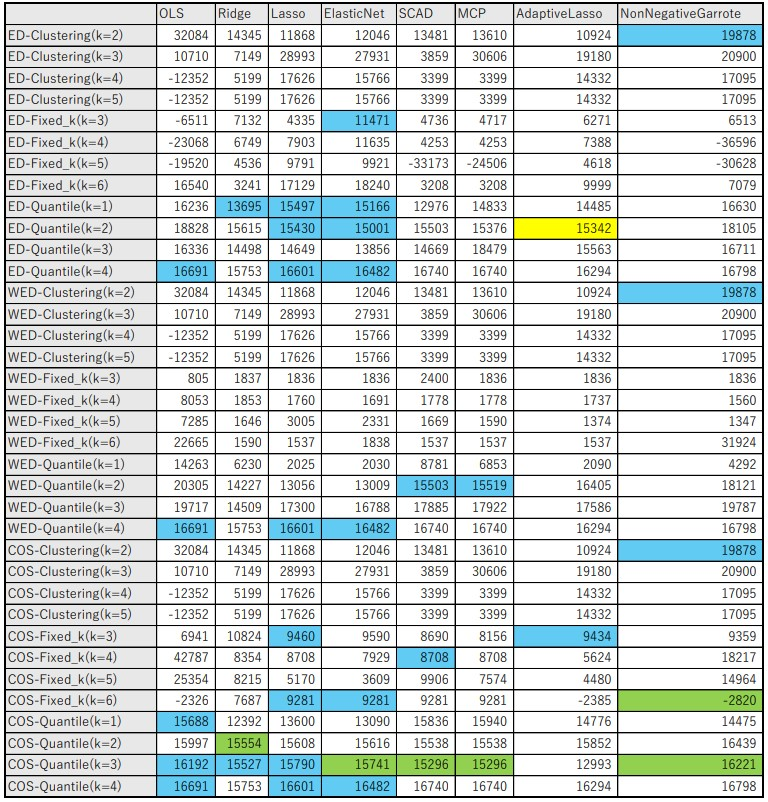
\includegraphics[width=120mm]{figure/fig/estDf_color.jpg}
  \captionsetup{labelformat=empty} % 図番号を非表示に設定
  \caption{\Fdualcaption{Colored ``Predicted Effort for New Project" Report.}{精度が高い手法の予測値}}
  \label{fig:estColor}
\end{figure}